\documentclass{article}

% use Times
\usepackage{times}
% For figures
\usepackage{graphicx} % more modern
%\usepackage{epsfig} % less modern
\usepackage{subfigure} 


% For citations
\usepackage{natbib}

% For algorithms
\usepackage{algorithm}
\usepackage{algorithmic}

% As of 2011, we use the hyperref package to produce hyperlinks in the
% resulting PDF.  If this breaks your system, please commend out the
% following usepackage line and replace \usepackage{icml2017} with
% \usepackage[nohyperref]{icml2017} above.
\usepackage{hyperref}

% Packages hyperref and algorithmic misbehave sometimes.  We can fix
% this with the following command.
\newcommand{\theHalgorithm}{\arabic{algorithm}}

% Employ the following version of the ``usepackage'' statement for
% submitting the draft version of the paper for review.  This will set
% the note in the first column to ``Under review.  Do not distribute.''
%\usepackage{icml2017} 

% Employ this version of the ``usepackage'' statement after the paper has
% been accepted, when creating the final version.  This will set the
% note in the first column to ``Proceedings of the...''
\usepackage[accepted]{icml2017}

% Stuff I added %%%%%%%%%%%%%%%%%%%%%%%%%%%%%%%
\usepackage{bm, amsmath}
\usepackage{amsfonts}

\usepackage{eqparbox}
\renewcommand\algorithmiccomment[1]{%
	\#\ \eqparbox{COMMENT}{#1}%
}
\newcommand{\diff}{\mathrm{d}}

%%%%%%%%%%%%%%%%%%%%%%%%%%%%%%%%%%%%%%%%



% The \icmltitle you define below is probably too long as a header.
% Therefore, a short form for the running title is supplied here:
\icmltitlerunning{IFT6269 Project - Latent Dirichlet Allocation}

\begin{document} 

\twocolumn[
\icmltitle{Probabilisitic Graphical Models IFT6269 Project \\ 
Latent Dirichlet Allocation}

% you can specify symbols, otherwise they are numbered in order
% ideally, you should not use this facility. affiliations will be numbered
% in order of appearance and this is the preferred way.
\icmlsetsymbol{equal}{*}

\begin{icmlauthorlist}
\icmlauthor{Patrice B\'echard}{equal,um}
\icmlauthor{Th\'eophile Gervet}{equal,mg}
\end{icmlauthorlist}

\icmlaffiliation{um}{Universit\'e de Montr\'eal, Montr\'eal, Canada}
\icmlaffiliation{mg}{McGill University, Montr\'eal, Canada}

\icmlcorrespondingauthor{Patrice B\'echard}{patrice.bechard@umontreal.ca}
\icmlcorrespondingauthor{Th\'eophile Gervet}{theophile.gervet@umontreal.ca}

% You may provide any keywords that you 
% find helpful for describing your paper; these are used to populate 
% the "keywords" metadata in the PDF but will not be shown in the document
\icmlkeywords{boring formatting information, machine learning, ICML}

\vskip 0.3in
]

% this must go after the closing bracket ] following \twocolumn[ ...
%]

% This command actually creates the footnote in the first column
% listing the affiliations and the copyright notice.
% The command takes one argument, which is text to display at the start of the footnote.
% The \icmlEqualContribution command is standard text for equal contribution.
% Remove it (just {}) if you do not need this facility.

%\printAffiliationsAndNotice{}  % leave blank if no need to mention equal contribution
\printAffiliationsAndNotice{\icmlEqualContribution} % otherwise use the standard text.

\begin{abstract} 
We present the generative probabilistic model of latent Dirichlet allocation useful for topic modeling on text corpora. We implement the model using two different algorithms to do approximate inference on the intractable posterior we want to estimate : variational inference and Gibbs sampling. Experiments on real data are conducted using the \textit{20 newsgroups} dataset. All the code is available online on GitHub : \url{https://github.com/patricebechard/Probabilistic_Graphical_Models_IFT6269}.
\end{abstract} 

\section{Introduction and Related Works}

\subsection{Latent Dirichlet Allocation}

\subsubsection{Generative Process}
Latent Dirichlet allocation (LDA) is a generative probabilisitic model of a corpus of $D$ documents $\{\mathbf{w}_1,..., \mathbf{w}_D\}$. Each document $\mathbf{w}_d = (w_{d,1},...,w_{d,N_d})$ is a sequence of $N_d$ words from a vocabulary indexed by $\{1,...,V\}$. 

The basic idea behind LDA is that each document is represented as a random mixture over $K$ latent topics, where each topic is characterized by a multinomial distribution over words, parametrized by a vector $\bm{\beta}_{k}$, $k \in {1,...,K}$. 

Formally, LDA assumes the following generative process for each document $\mathbf{w}_d$:
\begin{enumerate}
\item Sample a distribution over topics $\bm{\theta_d} \sim Dir(\bm{\alpha})$
\item For each of the $N_d$ words $w_{d,n}$ independently:
\begin{enumerate}
\item Draw a topic from the distribution over topics $z_{d,n} \sim \mathrm{Mult}(\bm{\theta}_d)$
\item Draw a word from this topic \\ 
$w_{d,n} \sim \mathrm{Mult}(\bm{\beta}_{z_{d,n}})$
\end{enumerate}
\end{enumerate}
This generative process is illustrated in the directed graphical model of figure \ref{graph_model}.



\begin{figure}[ht]
%\vskip 0.2in
\begin{center}
\centerline{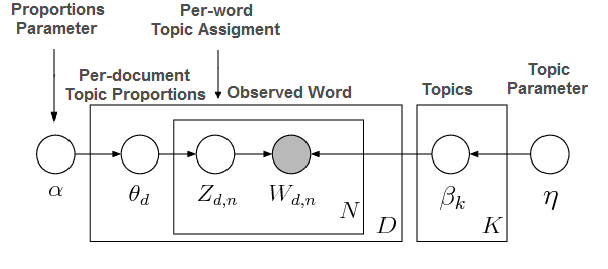
\includegraphics[width=\columnwidth]{LDA_graph_model}}
\caption{Graphical model corresponding to the generative process for LDA.}
\label{graph_model}
\end{center}
\vskip -0.2in
\end{figure} 

The joint distribution associated with this model is:
{\small
\begin{multline} 
	\label{joint}
	\prod_{k=1}^{K} p(\bm{\beta}_k | \bm{\eta}) 
	\prod_{d=1}^{D} p(\bm{\theta}_d | \bm{\alpha})
	\prod_{n=1}^{N_d} p(z_{d,n} | \bm{\theta}_d) p(w_{d,n} | z_{d,n}, \bm{\beta}_{1:K})
\end{multline}
}
where \\
$z_{d,n} \sim \mathrm{Mult}(\bm{\theta}_d)$, i.e $p(z_{d,n} | \bm{\theta}_d) = \theta_{d, z_{d,n}}$ \\
$w_{d,n} \sim \mathrm{Mult}(\bm{\beta}_{z_{d,n}})$, i.e $p(w_{d,n} | z_{d,n}, \bm{\beta}_{1:K}) = \beta_{z_{d,n},w_{d,n}}$ \\
$\bm{\beta}_k \sim \mathrm{Dir}(\bm{\eta})$ \\
$\bm{\theta}_d \sim \mathrm{Dir}(\bm{\alpha})$ \\

This generative process is just a model of the structure we assume to be in our data. In reality, we only observe documents $\mathbf{w}_{1:D}$ and our goal is to infer the underlying topic structure: the topics $\bm{\beta}_{1:K}$, the per document distributions over topics $\bm{\theta}_{d}$, and per document per word topic assignments $z_{d, n}$. 

Since the generative process assumes independence between documents, the probability of the whole corpus decomposes as a product of terms for individual documents. In order to clarify the notation, from now on let us consider equations for a single document $\mathbf{w}$ with $N$ words.

Assuming the Dirichlet hyper-parameters $\bm{\alpha}$ and $\bm{\eta}$ are fixed, we want to infer the posterior distribution:
\begin{equation}\label{eq:posteriorLDA}
 p(\bm{\beta}, \bm{\theta}, \mathbf{z} | \mathbf{w}, \bm{\alpha}, \bm{\eta}) =
 \frac{p(\bm{\beta}, \bm{\theta}, \mathbf{z}, \mathbf{w} | \bm{\alpha}, \bm{\eta})}{p(\mathbf{w} | \bm{\alpha}, \bm{\eta})}
\end{equation}

Unfortunately, this distribution is intractable to compute because the normalization factor $p(\mathbf{w} | \bm{\alpha}, \bm{\eta})$ cannot be computed exactly. We must use approximate inference to estimate the posterior over latent variables $\bm{\beta}$, $\bm{\theta}$ and $\mathbf{z}$. We will explore both variational inference and Gibbs sampling to solve this problem.

\subsection{Related Works}
Most of the work done in this article is based on the original Latent Dirichlet Allication paper \cite{blei2003latent}, which covers the general theory of the model as well as the variational inference approach to estimate the posterior. Other works present the Gibbs sampling approach for the same problem and provide useful implementation details \cite{darling2011theoretical, griffiths2002gibbs, heinrich2005parameter}.

Latent Dirichlet Allocation is an extension of the probabilistic latent semantic analysis (pLSA) model \cite{hofmann1999probabilistic}, which postulates that a document $\mathbf{w}$ and a word $w_{n}$ are conditionally independent given a latent topic $z$ :

\begin{equation*}
p(\mathbf{w},w_{n}) = p(\mathbf{w}) \sum_z p(w_n|z)p(z|\mathbf{w})
\end{equation*}

Some problems arise with this model. First, while it does make it possible for a document to contain multiple topics, the model only learns the topic mixtures $p(z|\mathbf{w})$ for the documents it has seen during the training, making it difficult to use it to assign probability to previously unseen documents. Furthermore, the number of parameters which the model tries to estimate grows linearly with the number of documents in the training set, which makes the model prone to overfitting. LDA overcomes both of the main problems with pLSA by adding a Dirichlet prior over the documents, defining a complete generative model.

However, LDA is by no means perfect. There have been many new ways to enhance the model to make it more realistic by relaxing some assumptions made by the model. The bag-of-words assumption is fine for our use of LDA, which is to uncover the topics present in a document and to assign a certain word to a topic. For more complicated goals, such as generating text, the assumption becomes inappropriate. There have been a number of extensions of the model that relax the bag-of-words assumption, for example, by combining the LDA with a Hidden Markov Model (HMM) to take into account the ordering of the words \cite{griffiths2005integrating}. It is also possible to relax the assumption that the ordering of the documents is irrelevant if we wish to find the evolution of certain topics over time, for example. A dynamic topic model would then be more appropriate than the classic LDA \cite{blei2006dynamic}.

\section{Algorithms}

\subsection{Variational EM}
To make our life easier, we derive a variational EM algorithm for a slightly simpler graphical model for LDA (the one presented in the original paper). We remove the Dirichlet prior over topics, this corresponds to removing the dependence of the $\bm{\beta}$ plate on the $\bm{\eta}$ random variable (see Figure \ref{graph_model2}, left). By doing so, we lose our ability to smooth topics through the $\bm{\eta}$ parameter.

Assuming the $\bm{\alpha}$ parameter and topics $\bm{\beta}$ are fixed, the posterior for a single document $\mathbf{w}$ now takes the form:
\begin{equation}
p(\bm{\theta}, \mathbf{z} | \mathbf{w}, \bm{\alpha}, \bm{\beta}) =
\frac{p(\bm{\theta}, \mathbf{z}, \mathbf{w} | \bm{\alpha}, \bm{\beta})}
		{p(\mathbf{w} | \bm{\alpha}, \bm{\beta})} 
\end{equation}

This expression is still intractable because of the denominator $p(\mathbf{w} | \bm{\alpha}, \bm{\beta})$. 

Let us motivate a variational EM algorithm by looking at how this intractable posterior comes back to bite us when we try to maximize the likelihood of the observed data. Since the probability of the whole corpus decomposes as a product of terms for individual documents, the log likelihood of the whole corpus decomposes as a sum of terms for individual documents. The log likelihood of a single document $\mathbf{w}$ takes the form:
\begin{equation}
\log p(\mathbf{w} | \bm{\alpha}, \bm{\beta}) =
	\log \int \sum_{\mathbf{z}} p (\bm{\theta}, \mathbf{z}, \mathbf{w} | \bm{\alpha}, \bm{\beta}) \diff\bm{\theta} 
\end{equation}

Because of the integral over $\bm{\theta}$ and the sum over $\mathbf{z}$ inside the log, we cannot maximize this objective directly. One common way to solve this problem is the Expectation Maximization (EM) algorithm. We make the following observation:
\begin{align*}
\log p(\mathbf{w} | \bm{\alpha}, \bm{\beta}) 
&= \log \int \sum_{\mathbf{z}} \frac{p (\bm{\theta}, \mathbf{z}, \mathbf{w} | \bm{\alpha}, \bm{\beta}) q(\bm{\theta}, \mathbf{z})}{q(\bm{\theta}, \mathbf{z})}  \diff\bm{\theta} \\
&= \mathbb{E}_q \left[\log \int \sum_{\mathbf{z}} \frac{p (\bm{\theta}, \mathbf{z}, \mathbf{w} | \bm{\alpha}, \bm{\beta})}{q(\bm{\theta}, \mathbf{z})}  \diff\bm{\theta}\right] \\
&\geq \mathbb{E}_q \left[\log p(\bm{\theta}, \mathbf{z}, \mathbf{w} | \bm{\alpha}, \bm{\beta})\right] - \mathbb{E}_q \left[\log q(\bm{\theta}, \mathbf{z})\right] \\
&= \mathcal{L}(q, \bm{\alpha}, \bm{\beta})
\end{align*}
where we have introduced an arbitrary distribution $q(\bm{\theta}, \mathbf{z})$ over the problematic latent variables $\bm{\theta}$ and $\mathbf{z}$, and the last step follows from Jensen's inequality.

The EM algorithm consists in alternatively maximizing the lower bound $\mathcal{L}$ on the log likelihood with respect to the distribution $q$ (the E-step), and with respect to parameters $\bm{\alpha}$ and $\bm{\beta}$ (the M-step).

One can easily show that maximizing $\mathcal{L}$ with respect to $q$ is equivalent to minimizing $\mathrm{KL}\left(q(\bm{\theta}, \mathbf{z}) || p(\bm{\theta}, \mathbf{z} | \mathbf{w}, \bm{\alpha}, \bm{\beta})\right)$. A simple solution is thus to set $q(\bm{\theta}, \mathbf{z})$ to be $p(\bm{\theta}, \mathbf{z} | \mathbf{w}, \bm{\alpha}, \bm{\beta})$, the true posterior over latent variables under the model.

In our case, things are not so simple: as we have seen, the posterior $p(\bm{\theta}, \mathbf{z} | \mathbf{w}, \bm{\alpha}, \bm{\beta})$ is intractable. This is were variational inference comes into play. The basic idea is to introduce a parametrized family of distributions over latent variables and phrase inference as an optimization problem. 

We parametrize $q$ as follows, according to the mean field independence assumption:
\begin{equation}
q(\bm{\theta}, \mathbf{z} | \bm{\gamma}, \bm{\phi}) =
q(\bm{\theta} | \bm{\gamma}) \prod_{n=1}^N q(z_n | \bm{\phi}_n)
\end{equation}
where the dirichlet parameters $\bm{\gamma}$ and the multinomial parameters $\bm{\phi}_n$, $n \in \{1,...,N\}$ are free variational parameters. The graphical model corresponding to this parameterization is illustrated in Figure \ref{graph_model2}, right.

\begin{figure}[ht]
\vskip 0.2in
\begin{center}
\centerline{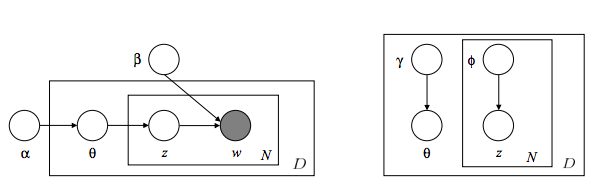
\includegraphics[width=\columnwidth]{LDA_graph_model2}}
\caption{(Left) Graphical model representation of LDA without prior over topics. (Right) Graphical model representation of the variational distribution used to approximate the posterior.}
\label{graph_model2}
\end{center}
\vskip -0.2in
\end{figure} 

Now variational inference consists in solving the following optimization problem:
\begin{equation}
(\bm{\gamma}^*, \bm{\phi}^*) =
\underset{\bm{\gamma}, \bm{\phi}}{\text{arg min}}\;
	\mathrm{KL}(q(\bm{\theta}, \mathbf{z} | \bm{\gamma}, \bm{\phi})~||~p(\bm{\theta}, \mathbf{z} | \mathbf{w}, \bm{\alpha}, \bm{\beta}))
\end{equation}

Note that $q(\bm{\theta}, \mathbf{z} | \mathbf{w}, \bm{\gamma}^*, \bm{\phi}^*)$ is actually a conditional distribution varying as a function of $\mathbf{w}$ because the optimization objective depends on $\mathbf{w}$. It can thus be seen as an approximation to the posterior $p(\bm{\theta}, \mathbf{z} | \mathbf{w}, \bm{\alpha}, \bm{\beta})$.

With this tool at our disposal, we can come back and complete the EM algorithm described in section 1.1.2. We can expand our variational lower bound on the per-document log likelihood as follows:
\begin{multline}
\mathcal{L}(\bm{\gamma}, \bm{\phi},\bm{\alpha}, \bm{\beta}) = 
\mathbb{E}_q [\log p(\bm{\theta} | \bm{\alpha})] + 
\mathbb{E}_q [\log p(\mathbf{z} | \bm{\theta})] + \\
\mathbb{E}_q [\log p(\mathbf{w} | \mathbf{z}, \bm{\beta})] -
\mathbb{E}_q [\log q(\bm{\theta} | \bm{\gamma})] -
\mathbb{E}_q [\log q(\mathbf{z} | \bm{\phi})]
\end{multline}
where the first three terms correspond to the expected complete log likelihood under $q$ and the last two terms to the entropy of $q$.

\subsubsection{E-step}
In the E-step, we maximize $\mathcal{L}$ with respect to the variational parameters $\bm{\gamma}$ and $\bm{\phi}$. This corresponds to applying the following update rules iteratively until convergence for each document:
\begin{equation} 
\label{phi_update}
\bm{\phi}_{n,k} \propto \bm{\beta}_{k, w_n} \exp\{\Psi(\bm{\gamma}_k)\}
\end{equation}
\begin{equation}
\label{gamma_update}
\bm{\gamma}_{k} = \bm{\alpha}_{k} + \sum_{n=1}^N \bm{\phi}_{n,k}
\end{equation}
where $\Psi(x) = \frac{\Gamma'(x)}{\Gamma(x)}$ is the digamma function.

Theses updates make sense intuitively. Equation \ref{phi_update} tells us that $\bm{\phi}_{n,k}$, the probability that word $w_n$ is generated by latent topic $k$, is proportional to the probability of drawing $w_n$ from topic $k$ times a quantity proportional to how much the document likes topic $k$ (the dirichlet parameter $\bm{\gamma}_k$). Equation \ref{gamma_update} tells us that the dirichlet parameter $\bm{\gamma}_k$ is equal to the pseudo-count $\bm{\alpha}_k$ given by the dirichlet prior plus the expected count of words picking topic $k$.

\subsubsection{M-step}
For the M-step, we maximize the overall variational lower bound with respect to parameter $\bm{\beta}$. We could also maximize with respect to $\bm{\alpha}$ but we chose to keep it fixed to make things simpler. As said before, the overall log likelihood of the corpus is the sum of the log likelihoods for the individual documents. Likewise, the overall variational lower bound is the sum of the individual variational bounds. 

Maximizing with respect to $\bm{\beta}$ gives the following update:
\begin{equation} 
\label{beta_update}
\bm{\beta}_{k,j} \propto \sum_{d=1}^D \sum_{n=1}^{N_d} \bm{\phi}_{d, n, k}
w_{d,n}^{(j)}
\end{equation}
where we abuse notation and index word $w_{d,n}$ which was a scalar until here as a one hot vector.

Equation \ref{beta_update} also has an intuitive meaning: the probability of word $j$ under topic $k$ is proportional to the expected count under the variational distribution of the number of times word $j$ is assigned topic $k$ across the whole corpus.

\subsubsection{Overall Algorithm}
We implemented a variational "EM flavored" algorithm which we described in detail in algorithm \ref{algo:EM}. Note that to be strictly an EM algorithm, we should maximize $\mathcal{L}$ with respect to $\bm{\phi}$ and $\bm{\gamma}$ all the way at each E-step. Instead, we alternate a single step of improvement with respect to the variational parameters with one step of improvement with respect to $\bm{\beta}$. Our algorithm has the same guarantee to increase the variational lower bound at each iteration, it is just more convenient to check for convergence only for the overall algorithm instead of for each E-step.

\begin{algorithm}[htb]
   \caption{Variational EM}
   \label{algo:EM}
\begin{algorithmic}
   \STATE {\bfseries Input:} documents $\mathbf{w}_1,...,\mathbf{w}_D$
   \STATE Set $\bm{\alpha}_k = 1 / K$ for all $k$ 
   \STATE Randomly initialize variational parameters $\bm{\gamma}$, $\bm{\phi}$ 
   \REPEAT
   \FOR{$d = 1$ {\bfseries to} $D$}
   \FOR{$k = 1$ {\bfseries to} $K$}
  	\FOR{$n = 1$ {\bfseries to} $N_d$}
  	\STATE $\bm{\phi}_{d,n,k} = \bm{\beta}_{k, w_n} \exp\{\Psi(\bm{\gamma}_{d,k})\}$
  	\ENDFOR
  	\STATE normalize $\bm{\phi}_{d,n}$ to sum to 1
  	\STATE $\bm{\gamma}_{d,k} = \bm{\alpha}_k + \sum_{n=1}^{N_d} \bm{\phi}_{d,n,k}$
   \ENDFOR
   \ENDFOR
   \FOR{$k = 1$ {\bfseries to} $K$}
   \FOR{$j = 1$ {\bfseries to} $V$}
   \STATE $\bm{\beta}_{k,j} = \sum_{d=1}^D \sum_{n=1}^{N_d} \bm{\phi}_{d, n, k} w_{d,n}^{(j)}$
   \ENDFOR
   \STATE normalize $\bm{\beta}_k$ to sum to 1
   \ENDFOR
   \STATE 
   \UNTIL{objective $\mathcal{L}$ doesn't improve anymore}
\end{algorithmic}
\end{algorithm}

\subsection{Gibbs Sampling}

Once again, we consider a single document $\mathbf{w}$ with $N$ words. Recall that we are interested in the latent topics $\bm{\beta}_{1:K}$, the distribution over topics $\bm{\theta}$, and the per word topic assignments $z_{n}$, $n \in \{1,...,N\}$. 

We could derive conditional distributions for each of these latent variables, and therefore an LDA Gibbs sampling algorithm, but we note that both $\bm{\theta}_{d}$ and $\bm{\beta}_k$ can be computed using the topic assignments $z_{d,n}$ which are sufficient statistics. This allows us to integrate out the multinomial parameters and simply sample $z_{d,n}$. This strategy is referred to as \textit{collapsed} or \textit{Rao-Blackwellized} Gibbs sampling \cite{heinrich2005parameter}.

The conditional we want to sample the topic assignment $z_n$ from is given by :

\begin{equation*}
p(z_n|\mathbf{z}_{\neg n}, \bm{\alpha}, \bm{\eta}, \mathbf{w})
\end{equation*}

where $\mathbf{z}_{\neg n}$ denotes all topic allocations except for $z_n$ and where we have reintroduced the hyperparameter $\bm{\alpha}$ controlling the topics-per-document proportions as well as the hyperparameter $\bm{\eta}$ controlling the probability of a word being assign to a topic. We can develop this expression using Bayes' rule:

\begin{equation}\label{eq:posterior1}
p(z_n|\mathbf{z}_{\neg n}, \mathbf{w}, \bm{\alpha}, \bm{\eta}) \propto p(w_n|z_n,\mathbf{z}_{\neg n}, \mathbf{w}_{\neg n}, \bm{\eta}) p(z_n|\mathbf{z}_{\neg n}, \bm{\alpha})
\end{equation}

where we have used the fact that $\mathbf{w}\!\!\perp\!\!\bm{\alpha}|\mathbf{z}$ and $\mathbf{z}\!\!\perp\!\!\bm{\eta}$. Now, let's develop each term of equation \ref{eq:posterior1} for a given topic assignment $z_n = k$:

\begin{align}\label{eq:term1}
&p(w_n|z_n=k, \mathbf{z}_{\neg n}, \mathbf{w}_{\neg n}) \nonumber\\
& \qquad = \int p(w_n|z_n=k, \bm{\beta}_k)p(\bm{\beta}_k|\mathbf{z}_{\neg n}, \mathbf{w}_{\neg n}) \diff \bm{\beta}_k \nonumber\\
& \qquad = \frac{n_{\neg n,k}^{(w_n)} + \bm{\eta}_n}{\sum_{n'=1}^{V}\left( n_{\neg n, k} ^{(w_{n'})} + \bm{\eta}_{n'}\right)}
\end{align}

\begin{align}\label{eq:term2}
&p(z_n=k|\mathbf{z}_{\neg n}) \nonumber\\
& \qquad = \int p(z_n=k|\theta_{\mathbf{w}_n}) p(\theta_{\mathbf{w}_n}|\mathbf{z}_{\neg n}) \diff \theta_{\mathbf{w}_n} \nonumber\\
& \qquad = \frac{n_{\neg n, k} ^{(\mathbf{w}_n)} + \bm{\alpha}_k}{\sum_{k'=1}^{(K)} \left( n_{\neg n, k'} ^{(\mathbf{w}_n)} + \bm{\alpha}_{k'} \right) }
\end{align}

The results obtained follow a $\mathrm{Dirichlet}\left(n_{\neg n,k}^{(w_n)} + \bm{\eta}_n\right)$ and a $\mathrm{Dirichlet}\left(n_{\neg n, k} ^{(\mathbf{w}_n)} + \bm{\alpha}_k\right)$, respectively. These distributions were obtained by the integration of the product between a Multinomial distribution and its Dirichlet conjugate prior. A detailed derivation of these equations is presented in \cite{heinrich2005parameter}.

Putting together equations \ref{eq:term1} and \ref{eq:term2}, we obtain the posterior distribution from which we sample a new topic assignment $z_n$ :

\begin{align}\label{eq:posterior_sampling}
& p(z_n=k|\mathbf{z}_{\neg n}, \mathbf{w}) \nonumber\\
& \qquad \propto \frac{n_{\neg n,k}^{(w_n)} + \bm{\eta}_n}{\sum_{n'=1}^{V}\left( n_{\neg n, k} ^{(w_{n'})} + \bm{\eta}_{n'}\right)}\frac{n_{\neg n, k} ^{(\mathbf{w}_n)} + \bm{\alpha}_k}{\sum_{k'=1}^{(K)} \left( n_{\neg n, k'} ^{(\mathbf{w}_n)} + \bm{\alpha}_{k'} \right) }
\end{align}

Finally, after the \textit{burn-in} period of the Gibbs sampling, we can find the expressions for the parameters we are looking for, namely the term-by-topic distribution $\bm{\beta}$ and the topic-by-document distribution $\bm{\theta}$ as such:


\begin{equation}\label{eq:beta_final}
\bm{\beta}_{k,n} = \frac{n_k ^{(w_n)} + \bm{\eta}_{t}}{\sum_{t=1}^{V} n_k ^{(t)} + \bm{\eta}_{t}}
\end{equation}

\begin{equation}\label{eq:theta_final}
\bm{\theta}_{d,k} = \frac{n_m ^{(k)} + \bm{\alpha}_k}{\sum_{k=1}^{K} n_m ^{(k)} + \bm{\alpha}_k}
\end{equation}

Algorithm \ref{algo:Gibbs} presents the various steps of the implementation of LDA using collapsed Gibbs sampling to estimate the posterior distribution.


\begin{algorithm}[htb]
   \caption{Gibbs Sampling}
   \label{algo:Gibbs}
\begin{algorithmic}
   \STATE {\bfseries Input:} documents $\mathbf{w}_1,...,\mathbf{w}_D$   
   \STATE Initialize hyperparameters $\bm{\alpha}$ and $\bm{\eta}$
   \STATE Randomly initialize topic assignments $z_{d,n}$ for all $d$, $n$
   \STATE Increment counters $n_{d,k}$ and $n_{k,n}$
   \REPEAT
   \FOR{$d = 1$ {\bfseries to} $D$}
  	  \FOR{$n = 1$ {\bfseries to} $N_d$}
  	  \STATE $n_{d,z_{d,n}} -\!\!= 1;\quad n_{z_{d,n},n} -\!\!= 1$
	  %\STATE $p(z=k|\cdot) = (n_{d,k} + \bm{\alpha}_k)\frac{n_{k,n} + \bm{\beta}_n}{\sum_{n'=1}^{N} n_{k,n'} + \bm{\beta}_{n'}}$
	  %\STATE Sample topic assignment $z_{d,n} \sim p(z=k|\cdot)$
	  \STATE Sample topic assignment $z_{d,n}$ from equation \ref{eq:posterior_sampling}
	  \STATE $n_{d,z_{d,n}} +\!\!= 1;\quad n_{z_{d,n},n} +\!\!= 1$
  	  \ENDFOR
   \ENDFOR
   \UNTIL{convergence}
   \STATE compute $\bm{\beta}_{k,n}$ from equation \ref{eq:beta_final} for all $d$, $k$
   \STATE compute $\bm{\theta}_{d,k}$ from equation \ref{eq:theta_final} for all $k$, $n$

\end{algorithmic}
\end{algorithm}



\subsubsection{Choice of hyperparameters}

Both $\bm{\alpha}$ and $\bm{\eta}$ are hyperparameters for our model. Typically, the a priori assumption of LDA is that all words are equally likely to be assigned to a topic, and all topics have equal chance of being assigned to a document. In this case, values of $50/K$ for each component of $\bm{\alpha}$ and $0.01$ for each component of $\bm{\eta}$ have been reported to yield good results \cite{griffiths2004finding}.

\section{Experimental Methods}
For experiments with both implementations of LDA, we used the \textit{20 Newsgroups} dataset \cite{20_newsgroups}. We train the models on a subset of the dataset, and assess generalization to unseen data using the \textit{perplexity} metric. In order to infer the distribution over topics for documents unseen during training (the $\bm{\theta}$ parameter) with Gibbs sampling, we use a method called query sampling. With the model trained with variational EM, we simply use variational inference. 

\subsection{Dataset and Preprocessing}
The \textit{20 Newsgroups} dataset contains approximately 20,000 newsgroup documents, partitioned nearly evenly across 20 different newsgroups, each corresponding to a different subject. Some of the newsgroups are very closely related to each other while others are unrelated. Figure \ref{20_newsgroups} roughly partitions the 20 newsgroups by subject matter. 

We use the train-test partition provided by sklearn (60\%-40\%), and preprocess the data by tokenizing, removing stop-words and punctuation, lemmatizing with the WordNetLemmatizer from the nltk library, and keeping only the 3000 most frequent words.

\begin{figure}[ht]
\vskip 0.2in
\begin{center}
\centerline{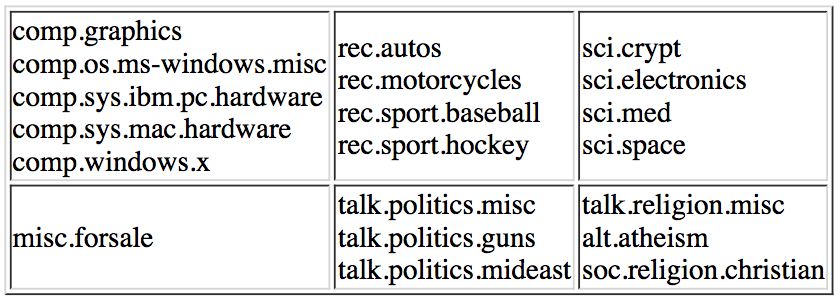
\includegraphics[width=\columnwidth]{20_newsgroups}}
\caption{Newsgroups classified by overlap in subjects}
\label{20_newsgroups}
\end{center}
\vskip -0.2in
\end{figure} 


\subsection{Perplexity}
Perplexity is a measure of the generalization performance of models and is used by convention in language modeling. It is defined algebraically as the inverse of the geometric mean per-word likelihood. A lower perplexity score indicates a better generalization performance for a model. For a test set of $D$ documents, the perplexity is given by :

\begin{align}\label{eq:perplexity}
\mathrm{perplexity}(D_{\mathrm{train}}) & = \sum_{d=1}^{D} p(\mathbf{w_d})^{-1/N_d} \nonumber\\
										& = \exp\left[-\frac{\sum_{d=1}^D \log p(\mathbf{w}_d)}{\sum_{d=1}^D N_d}\right]
\end{align}

For LDA, the likelihood found $p(\mathbf{w}_d)$ found in equation \ref{eq:perplexity} can be expressed as the parameters $\bm{\beta}$ and $\bm{\theta}$. If we develop the expression for the likelihood, we have :

\begin{align}
p(\mathbf{w}_d) & = \prod_{n=1}^{N_d} \sum_{k=1} ^K p(w_{d,n}=t|z_{n,d}=k) \nonumber \\
				& \qquad \qquad \qquad \qquad \cdot p(z_{d,n}=k|d=d) \nonumber\\
				& = \prod_{t=1}^{V} \left( \sum_{k=1}^K \bm{\beta}_{k,t} \cdot \bm{\theta}_{d,k} \right)^{n_d ^{(t)}}\nonumber\\
\log p(\mathbf{w}_d) & = \sum_{t=1}^V n_d ^{(t)} \log \left( \sum_{k=1}^K \bm{\beta}_{k,t} \cdot \bm{\theta}_{d,k} \right)
\end{align}

Here, $n_d ^{(t)}$ is the number of times term $t$ appears in document $d$. Note here that the term $\bm{\theta}_{d,k}$ has to be obtained for the new test documents via methods shown in the subsequent sections.

\begin{table*}[htb]
\caption{\label{tab:top_words_LDA} Most probable words associated to some topics for LDA trained with variational EM.}
\vskip 0.15in
\begin{center}
\begin{small}
\begin{tabular}{c|c|c|c|c|c|c|c|c|c|c|c}
\textsc{Space} & \textsc{Computer} & \textsc{Religion} & \textsc{Numbers} & \textsc{Mid-East} & \textsc{Sport}\\
\hline 
space & use & god & 10 & armenian & game\\
nasa & windows & people & 00 & people & team \\
program & file & believe & 25 &  jews & year  \\
earth & card & jesus & 15 &  turkish & games \\
launch & window & know & 11 &  war & time 
\end{tabular}
\end{small}
\end{center}
\label{default}
\end{table*}%

\subsection{Query sampling}

In order to infer the distribution over topics for documents unseen during training (the $\bm{\theta}$ parameter) with Gibbs sampling, we use a method called query sampling.

We consider the query (vector of words) $\tilde{\mathbf{w}}$ (note that we can have multiple queries at the same time, but we only consider one here for simplicity). Normally, the task of querying consists of finding similarity between the query and other documents by estimating the posterior distribution $\tilde{\mathbf{z}}$ given the query and the state of the LDA at the end of the training (represented by the Markov state $\bm{\mathcal{M}}=\{ \mathbf{z},\mathbf{w} \}$). Here, we want to find this distribution to compute the perplexity of our model. The algorithm is pretty straightforward and consists of assign topics randomly to words in $\tilde{\mathbf{w}}$ and to perform a certain number of loops through Gibbs sampling update on our query only. The distribution from which we sample $\tilde{z}$ from is given below :

\begin{align}\label{eq:posterior_query}
& p(\tilde{z}_n=k|\tilde{w}_n=t, \tilde{\mathbf{z}}_{\neg n},\tilde{\mathbf{w}}_{\neg n};\bm{\mathcal{M}}) \nonumber\\
& \quad = \frac{n_k ^{(t)} + \tilde{n}_{k, \neg n} ^{(t)} + \bm{\eta}_t}{\sum_{t'=1}^V n_k ^{(t')} + \tilde{n}_{k, \neg n} ^{(t')} + \bm{\eta}_t'} \cdot \frac{n_{\tilde{d},\neg n}^{(k)} + \bm{\alpha}_k}{\sum_{k'=1}^K n_{\tilde{d}^{(k')}} + \bm{\alpha}_k'}
\end{align}

where $\tilde{n}_k ^{(t)}$ is the number of observations of term t and topic k in the query. With this posterior distribution, we obtain the topic-per-document distribution for the document:

\begin{equation}
\bm{\theta}_{\tilde{m},k} = \frac{n_{\tilde{m}}^{(k)} + \bm{\alpha}_k}{\sum_{k'=1}^K n_{\tilde{m}}^{(k')} + \bm{\alpha}_k'}
\end{equation}

It is important that the size of the unknown documents be smaller than the training set, because the posterior (equation \ref{eq:posterior_query}) distorts the topic distribution obtained from the training.

\section{Results}

\subsection{Choosing the Number of Topics}
We pick the number of topics which gives the best generalization performance (the best test-set perplexity). 

For the variational inference implementation, we ran into some numerical issues to compute the likelihood of documents. Thus we computed training and test set perplexity with the batch variational inference implementation by sklearn. As we can see in figure \ref{perplexity}, training-set perplexity always goes down when we increase the number of topics, but the best test-set perplexity is attained for 12 topics. Overfitting occurs when more topics are chosen.

\begin{figure}[ht]
%\vskip 0.2in
\begin{center}
\centerline{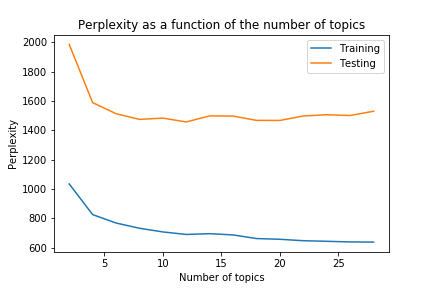
\includegraphics[width=\columnwidth]{perplexity_as_a_function_of_number_of_topics}}
\caption{Variational inference implementation: the best test set perplexity is reached at 12 topics.}
\label{perplexity}
\end{center}
\vskip -0.2in
\end{figure} 

TODO add similar curve for implementation with Gibbs sampling

\subsection{Visual Inspection of Topics}
We trained both our models with 12 topics in order to visually inspect the learnt topics. The most probable words for each topic for LDA trained with our model of variational EM are in table \ref{tab:top_words_LDA}. We only present the 6 most relevant topics for each model. The most probable words for each topic for LDA trained using collapsed Gibbs sampling are presented in table \ref{tab:top_words_LDA_gibbs}. 

\begin{table*}[htb]
\caption{\label{tab:top_words_LDA_gibbs} Most probable words associated to some topics for LDA trained with collapsed Gibbs sampling.}
\vskip 0.15in
\begin{center}
\begin{small}
\begin{tabular}{c|c|c|c|c|c|c|c|c|c|c|c}
\textsc{Space} & \textsc{Computer} & \textsc{Religion} & \textsc{Numbers} & \textsc{Mid-East} & \textsc{Sport}\\
\hline 
space & drive & god & 1 & armenian & game\\
nasa & card & jesus & 2 & jew & year \\
mission & disk & christ & 0 &  turkish & team  \\
data & system & life & 3 &  muslim & run \\
lunar & controller & sin & 4 &  people & player 
\end{tabular}
\end{small}
\end{center}
\label{default}
\end{table*}%



\section{Discussion}

In this report, we have presented the generative process assumed in the latent Dirichlet allocation. Because of an intractable posterior, approximate inference was needed to compute the desired quantities. Variational inference as well as Gibbs sampling were used to approximate the posterior. We also conduct experiments on text data from the \textit{20 newsgroups} dataset and present the obtained perplexity and most probable words found for certain topics for each model. Although latent Dirichlet allocation is one of the most simple and useful models for topic modeling, its generative process is not really realistic, relying on the bag of words assumption. More recently, Hidden Topic Markov Model \cite{gruber2007hidden} and many other probabilistic graphical models have tried to relax this assumption.

% In the unusual situation where you want a paper to appear in the
% references without citing it in the main text, use \nocite
\nocite{blei2012probabilistic}

\bibliographystyle{icml2017}
\bibliography{report}

\end{document} 


% This document was modified from the file originally made available by
% Pat Langley and Andrea Danyluk for ICML-2K. This version was
% created by Lise Getoor and Tobias Scheffer, it was slightly modified  
% from the 2010 version by Thorsten Joachims & Johannes Fuernkranz, 
% slightly modified from the 2009 version by Kiri Wagstaff and 
% Sam Roweis's 2008 version, which is slightly modified from 
% Prasad Tadepalli's 2007 version which is a lightly 
% changed version of the previous year's version by Andrew Moore, 
% which was in turn edited from those of Kristian Kersting and 
% Codrina Lauth. Alex Smola contributed to the algorithmic style files.  
